\chapter{Background and Related Work}
In the following chapter the background necessary for the Bayesian Markov Blanket Estimation and its extension with Simulated Annealing is provided.
First, the statistical methods used for the inference of our models are covered.
This includes \gls{MCMC} sampling for the estimation of the whole posterior distribution and Simulated Annealing for a \gls{MAP} estimate.
Subsequently, copulas and more specifically the semi parametric Gaussian copula are presented.
Copulas allows generalizing the \gls{BMB} and similar models to mixed data by introducing latent variables and relaxing the assumptions about the marginal distributions of the data.
At last we introduce Gaussian Graphical Models and the matters of their estimation in a high-dimensional setting.


\section{Markov Chain Monte Carlo}
This section is mainly based on \citet{andrieu2003introduction}, which provides an overview and introduction to \gls{MCMC} methods.

Bayesian inference allows us to update our prior beliefs when observing data to produce our posterior belief.
Let $\matr{\theta}$ be the parameters of a statistical model and $X$ the observed data distributed according to the (unknown) \gls{pdf} $p(X)$.
The Likelihood $p(X|\theta)$ then quantifies how 'likely' it is, that data $X$ was created according to the statistical model parametrized by $\theta$.
Preexisting and arguably subjective beliefs we have about the parameters are captured in the prior \gls{pdf} $p(\theta)$. 
When observing data $X$, the prior can then be updated to the posterior according to the well known Bayes' Theorem \cite[Chapter 1.2.3]{Bishop:2006:PRM:1162264}:
$$
p(\theta|X) = \frac{p(X|\theta) p(\theta)}{p(X)} =  \frac{p(X|\theta) p(\theta)}{\int_\Theta p(X|\theta')p(\theta') d\theta'}
$$
The posterior \gls{pdf} then expresses our uncertainty about $\theta$, while incorporating both the observed data and our prior beliefs.
Although the posterior can be given as a closed-form expression in special cases (e.g. by using conjugate priors), this is generally not the case.
The main difficulty arises from the unknown $p(X)$.
Although it can be calculated by marginalization, the integral usually offers no analytical solution, and numerical integration is computationally intractable for even moderately large parameter spaces.
For tackling this problem, \gls{MCMC} methods can be used.
MCMC techniques provide a framework for sampling from target distributions which can be evaluated up to a normalizing constant.
As such, the posterior distribution can be empirically estimated without the need to explicitly compute the prohibitively large normalization.

Because the posterior need be known only up to a constant, knowing the likelihood $p(X|\theta)$ and the prior $p(\theta)$ is sufficient:
$$
p(\theta|X) = \frac{p(X|\theta)p(\theta)}{\int_\Theta p(X|\theta')p(\theta') d\theta'} \propto p(X|\theta)p(\theta)
$$

Sampling from a target distribution is achieved by constructing homogeneous, 'irreducible and aperiodic Markov chains that have the target distribution as the invariant distribution' \citep{andrieu2003introduction}.
That is, the chain must not have any cycles (\textit{aperiodicity}) and every state with non-zero probability must be reachable within a finite number of steps (\textit{irreducibility}).
A sufficient (but not necessary) condition for having a specific distribution $p(x)$ as the invariant distribution of a discrete Markov chain with transition matrix $T$ is the \textit{detailed balance} property (\cite[Chapter 11.2.1]{Bishop:2006:PRM:1162264}):
\begin{equation}
	\label{eq:mcmc_invar}
	p(x^{(i)})T(x^{(i-1)} | x^{(i)})=  p(x^{(i-1)})T(x^{(i)} | x^{(i-1)})
\end{equation}
By constructing a Markov chain that satisfies these conditions, a corresponding sampler can then be constructed.
The empirical distribution of the samples drawn from the chain then converges \textit{almost surely} to the target distribution, which in our case is the posterior distribution.
But while convergence itself might be a.s. guaranteed for $n\rightarrow \infty$, the convergence rate
strongly depends on the specific Markov chain used. So while fulfilling the necessary conditions might be sufficient in theory, a Markov chain with quick convergence is required in practice.
In the following subsections we will present two well known MCMC techniques for sampling from a target distribution.
 
\subsection{Metropolis Hastings}
Metropolis Hastings (MH) is a \gls{MCMC} method introduced by \citet{hastings1970monte}.
While we do not directly make use of a \gls{MH} sampler in the presented models, \gls{MH} can be viewed as a general case of other samplers. 
As we'll show in the following sections, this will be useful for extending a Gibbs Sampler for Simulated Annealing.

The \gls{MH} procedure is based on drawing samples from a proposal function and then randomly accepting or rejecting them as draws from the target distribution.
Let $p(x)$ be the invariant distribution we are interested in (known up to a constant) and $q(x^*|x)$ some proposal function. The proposal function suggests a new candidate for our sampler, given a current value.
Unlike the Metropolis sampler \citep{metropolis1953equation}, \gls{MH} does not require the proposals to be symmetric.
\begin{algorithm}[H]
	\caption{Metropolis-Hastings Sampler}\label{alg:MH}
	\begin{algorithmic}
		\State \textbf{Initialize}: $x^{(0)}$
		\For{$i=0$ to $N-1$}
		\State Sample $u\sim \mathcal{U}_{[0,1]}$
		\State Sample $x^* \sim q(x^*|x^{(i)})$
		\If{$u< \mathcal{A}(x^{(i)}, x^*) = 
			\min 
			\Big\{ 
			1, \frac{p(x^*)q(x^{(i)} | x^*)}
			{p(x^{(i)})q(x^*|x^{(i)})} 
			\Big\} $}
		\State $x^{(i+1)} = x^*$
		\Else
		\State $x^{(i+1)} = x^{(i)}$
		\EndIf
		\EndFor
	\end{algorithmic}
\end{algorithm}

In Algorithm \autoref{alg:MH} the general sampler for which the Markov chain admits $p(x)$ as the invariant distribution is shown.
By construction, the transition probabilities of the \gls{MH} sampler satisfy \autoref{eq:mcmc_invar}. 
The aperiodicity of the chain is given by the possibility of rejection in the sampler.
For guaranteeing irreducibility, it need only be ensured that the proposal function $q(x*|x)$ has the same support as $p(x)$ (i.e. can lead to all states $x^*$ that have non-zero probability $p(x^*)$).
It should be noted, that $p(x)$ need be known only up to a constant. 
This follows from the fraction $\frac{p(x^*)q(x^{(i)} | x^*)}
{p(x^{(i)})q(x^*|x^{(i)})} $ which is not affected by a constant factor in $p(x)$.
While \gls{MH} is a very general method, its performance largely depends on the proposal function.
If the proposals are too conservative (i.e. if there are only very small changes compared to the previous sample), exploring the whole posterior will take a long time.
Conversely a proposal function that jumps around a lot may suffer from a low acceptance ratio, as many improbable values are considered.


\subsection{Gibbs Sampling}
\label{ss:Gibbs}
Gibbs sampling \citep{geman1984stochastic} is an MCMC method that can be applied if the target distribution is multivariate.
Instead of the joint distribution, it relies on the individual conditional distributions and is especially useful if the conditionals are known and easy to sample from.

Let $p(\matr{x}) = p(x_1, \dots, x_n)$ be the distribution we wish to sample from,
where the conditionals $$p(x_j|x_{-j}) = p(x_j | x_1, \dots x_{j-1}, x_{j+1}, \dots, x_n) \quad \quad \forall j \in \{1,\dots,n\}$$ are known.
By now iteratively drawing samples from the individual distributions while conditioning on the latest drawn samples of the other parameters, we can approximate the joint posterior $p(x_1,\dots,x_n)$.
This is convenient since the posterior conditionals can often be expressed in terms of a known closed form distribution (by using semi-conjugate priors), even if the full posterior cannot.

The Gibbs sampler can be viewed as a special case of Metropolis Hastings with the following distribution for the proposal function \citep{andrieu2003introduction}:
$$
q(x^*|x^{(i)}) = 
\left\{
\begin{array}{ll}
	p(x^*_j|x^{(i)}_{-j}) & \text{If } x^*_{-j} = x^{(i)}_{-j} 
	\\
	0                     & \text{otherwise}                   
\end{array}
\right.
$$

Substituting this into Algorithm \autoref{alg:MH} and using $p(x) = p(x_j|x_{-j}) p(x_{-j})$
leads to \cite[p. 544]{Bishop:2006:PRM:1162264}
$$
\mathcal{A}(x^{(i)}, x^*) = 
\min 
\Big\{ 
1, \frac{ p(x^*_j|x^*_{-j}) p(x^*_{-j}) p(x_j|x^*_{-j})}
{  p(x_j|x_{-j}) p(x_{-j}) p(x^*_j | x_{-j})  } 
\Big\} 
= 1
$$
Thus, the Gibbs sampler is a \gls{MH} sampler with acceptance probability $1$.
This perspective can now be used for incorporating Simulated Annealing on top of a Gibbs sampler, for which the posterior conditionals are available in closed forms.

The general sampler is shown in Algorithm \autoref{alg:Gibbs}.
Each iteration of it corresponds to a Gibbs sweep, where a new sample is drawn for each variable while conditioning on the most recent samples of the other variables.
Thus,  one draw from the joint distribution is obtained with each Gibbs sweep.
It should be noted, that the order of the variables does not influence the sample distribution for a sufficiently large number of iterations.
\begin{algorithm}[H]
	\caption{Gibbs Sampler}\label{alg:Gibbs}
	\begin{algorithmic}
		\State \textbf{Initialize}: $x_{0, 1:n}$
		\For{$i=0$ to $N-1$}
		\State Sample $x_1^{(i+1)}\sim p(x_1|x_2^{(i)}, x_3^{(i)}, \dots, x_n^{(i)})  $
		\State Sample $x_2^{(i+1)}\sim p(x_2|x_1^{(i+1)}, x_3^{(i)}, \dots, x_n^{(i)})  $
		\\
		\State \vdots
		\\
		\State Sample $x_j^{(i+1)}\sim p(x_j|x_1^{(i+1)}, x_{j-1}^{(i+1)},x_{j+1}^{(i)}, \dots, x_n^{(i)})  $
		\\
		\State \vdots
		\\
		\State Sample $x_n^{(i+1)}\sim p(x_n|x_1^{(i+1)}, x_2^{(i+1)}, \dots, x_{n-1}^{(i+1)})  $
		\EndFor
	\end{algorithmic}
\end{algorithm}

\FloatBarrier


\subsection{Simulated Annealing}
\label{ss:SA}
If we are only interested in a point estimation of the parameters, 
inferring the whole posterior distribution might not be the best solution.
Unless the area surrounding the mode of the posterior has a high amount of probability mass, the sampler will mainly explore areas that are of low interest.
Instead we can try to directly find the mode of the posterior, i.e. the \gls{MAP}.
Simulated Annealing \citep{kirkpatrick1983optimization} is an optimization framework that can be used for finding the global maximum of a given function.
The concept stems from metallurgy, where slowly cooling a previously heated material leads to it reaching an 'optimal' minimum energy state.


For applying \gls{SA} in the context of \gls{MCMC} sampling, we switch to a inhomogeneous Markov chain with the invariant distribution
$$ p_i (x) \propto p^{1/T_i} $$
where $T_i$ is the temperature at iteration $i$. 

Initially the temperature is very high, such that large jumps between the drawn samples are possible (as the invariant distribution will be very flat). 
The temperature is then slowly decreased, such that the distribution becomes more peaked and less jumping is possible. 
Eventually the invariant $p^{1/T_i}(x)$ tends to $p^\infty(x)$ for $lim_{i\rightarrow \infty}T_i=0$, which concentrates on the global maxima.
The concrete value of $T_i$ and its speed of decrease are defined by a cooling schedule $f_T(i)$. 
Convergence to the set of global maxima has been shown to hold for logarithmic cooling schedules in discrete domains \citep{geman1984stochastic}.
Unfortunately, a logarithmic cooling schedule is not a computationally feasible option for realistic problem sizes.
In the literature, a range of cooling schedules has been analyzed (e.g. \citet{abramson1999simulated}), but to our knowledge there is not one distinct cooling method that works best in practice.
In general, slower cooling of the system is preferred and the decrease in temperature should slow down with the temperature going towards 0.
A simple method that is quite popular in practice is a geometric cooling schedule
(see for example \cite{andrieu2000simulated, yuan2004annealed}).

\begin{tcolorbox}[title=Geometric Cooling Schedule (1)]
	Let $T_0$ be the initial temperature, $a\in\mathbb{R}_{> 0}$ be a constant.
	Then the temperature $T_i$ at iteration $i$ is:
	$$
	T_i = f_T(i) = T_0\  a^{i} \quad \quad i = 0,1,\dots,n
	$$
\end{tcolorbox}

Furthermore, as $\frac{1}{T}$ can never reach infinity in practice, one can set a (low) target temperature $T_n$, which is reached after $n$ iterations.
Adapting the geometric cooling schedule to reach a final temperature $T_n$ leads to:
\begin{tcolorbox}[title=Geometric Cooling Schedule (2)]
	\begin{equation}
		f_T(i) = T_0  \Big(\frac{T_n}{T_0}\Big)^{i/n} \quad \quad i = 0,1,\dots,n
	\end{equation}
\end{tcolorbox}
The form of the geometric cooling schedule can be seen in \autoref{fig:cool_exp}.
\begin{figure}
	\centering
	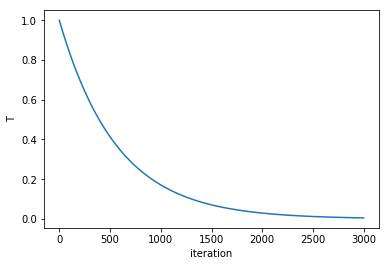
\includegraphics[width=0.5\textwidth]{cool_exp}
	\caption{Geometric cooling schedule for $T_n=0.005$, $T_0=1$ and $n=3000$}
		
	\label{fig:cool_exp}
\end{figure}

At the target temperature we can continue sampling from the invariant distribution $p^{1/T_n}(x)$. 
If convergence was achieved (i.e. if the cooling was slow enough) samples from this target temperature will be close to the true mode with high probability.
For estimating the final value, we can then for example look at statistics such as the median, mean or the credible intervals of the samples.
The Annealing can be implemented by slightly altering the \gls{MH} sampler, such that the invariant distribution at each step is $p^{1/T_i}(x)$, where the temperature $T_i$ is set according to the cooling schedule $f_T(i)$ (see Algorithm \autoref{alg:SA_MH}).


\begin{algorithm}[H]
	\caption{Simulated Annealing: Metropolis-Hastings}\label{alg:SA_MH}
	\begin{algorithmic}
		\State \textbf{Initialize}: $x^{(0)}$, $T_0=1$
		\For{$i=0$ to $N-1$}
				
		\State $T_{i} = f_T(i)$
		\\
		\State Sample $u\sim \mathcal{U}_{[0,1]}$
		\State Sample $x^* \sim q(x^*|x^{(i)})$
		\If{$u< \mathcal{A}(x^{(i)}, x^*) = 
			\min 
			\Big\{ 
			1, \frac{p(x^*)^{1/T_i} q(x^{(i)} | x^*)}
			{p(x^{(i)})^{1/T_i}q(x^*|x^{(i)})} 
			\Big\} $}
		\State $x^{(i+1)} = x^*$
		\Else
		\State $x^{(i+1)} = x^{(i)}$
		\EndIf
		\EndFor
	\end{algorithmic}
\end{algorithm}
Similar to \autoref{ss:Gibbs}, it is possible to use the conditional distributions as proposals:
$$
q(x^*|x^{(i)}) = 
\left\{
\begin{array}{ll}
	p(x^*_j|x^{(i)}_{-j})^{1/T_i} & \text{If } x^*_{-j} = x^{(i)}_{-j} 
	\\
	0                             & \text{otherwise}                   
\end{array}
\right.
$$
As before, one can show that this leads to an acceptance probability of 1 when input into Algorithm \autoref{alg:SA_MH}.
In consequence we can formulate the Simulated Annealing for a Gibbs sampler as shown in Algorithm \autoref{alg:SA_Gibbs}.

\begin{algorithm}[H]
	\caption{Simulated Annealing: Gibbs Sampler}\label{alg:SA_Gibbs}
	\begin{algorithmic}
		\State \textbf{Initialize}: $x_{0, 1:n}$, $T_0=1$
		\For{$i=0$ to $N-1$}
		\State $T_{i} = f_T(i)$
		\\
		\State Sample $x_1^{(i+1)}\sim p(x_1|x_2^{(i)}, x_3^{(i)}, \dots, x_n^{(i)})^{1/T_i}  $
		\State Sample $x_2^{(i+1)}\sim p(x_2|x_1^{(i+1)}, x_3^{(i)}, \dots, x_n^{(i)})^{1/T_i}  $
		\\
		\State \vdots
		\\
		\State Sample $x_j^{(i+1)}\sim p(x_j|x_1^{(i+1)}, x_{j-1}^{(i+1)},x_{j+1}^{(i)}, \dots, x_n^{(i)})^{1/T_i}  $
		\\
		\State \vdots
		\\
		\State Sample $x_n^{(i+1)}\sim p(x_n|x_1^{(i+1)}, x_2^{(i+1)}, \dots, x_{n-1}^{(i+1)})^{1/T_i} $
		\EndFor
	\end{algorithmic}
\end{algorithm}

\section{Semi-Parametric Gaussian Copula}
\label{s:semi_copula}
In many problem settings it is common to have mixed data for which we cannot assume a specific (closed form) marginal distributions,
while we still would like to assume a joint distribution of the data.
However, a model that would for example be based on multivariate Gaussian data also relies on univariate Gaussian marginals.
A solution for this is provided by Sklar's theorem \citep{sklar1959fonctions}, which says that a $p$-dimensional joint distribution can be represented in two parts: The $p$ marginal distributions and a \textit{copula} function, which describes the dependencies between the variables.
\begin{tcolorbox}[colback=yellow!5!white,colframe=yellow!75!black, title=Sklar's Theorem]
	\begin{customthm}{}[extracted from \citet{nadarajah2018compendium}]
		\label{th:sklar}
		Let \textit{F} be a \textit{p}-dimensional cumulative distribution function with marginal distribution functions $F_i, i=1,\dots,p$. Then there exists a copula C such that
		$$
		F(x_1,\dots,x_p) = C(F_1(x_1), \dots, F_p(x_p))
		$$
		Conversely, for any univariate cumulative distribution functions 
		$F_1,\dots, F_p$
		and any copula $C$, the function $F$ is a $p$-dimensional \gls{cdf} with marginals $F_1,\dots,F_p$. 
		Furthermore, if $F_1, \dots, F_p$are continuous, then C is unique.
	\end{customthm}
\end{tcolorbox}
So with the use of copulas, it is possible to parametrize the marginal distributions separately from their joint distribution. 
Consequently the dependency structure of the data can be assumed to follow a specific joint distribution (e.g. a multivariate Gaussian) without having to consider the unknown marginals.
It should be noted that Sklar's Theorem guarantees the uniqueness of the copula only where marginals are continuous.

Let $y_{i,j}$ be the $i$-th observation of variable $\matr{y}_j$, with $i=1,\dots,n$ and $j=1,\dots,p$.
For modeling the copula, latent variables $\matr{z}_j$ that are distributed according to the assumed joint distribution are introduced. 
The observed variables $y_{i,j}$ can then be represented as the result of a non-decreasing transformation $g_j(z_{i,j})$ of the latent data.
In the case of Gaussian copula models we assume that the latent variables are distributed according to a multivariate Normal distribution and can be modeled as follows
\citep{hoff2009first}.
\begin{tcolorbox}[colback=yellow!5!white,colframe=yellow!75!black, title=Gaussian Copula: Latent Normal Model]
	Let $\matr{z}_1, \dots, \matr{z}_n$ be $i.i.d.$ (latent) random variables drawn from a p-variate normal distribution, with $\matr{C}$ being a $p\times p$ correlation matrix.
	Furthermore, let $\matr{y}_j$ be the observed variables with marginal \gls{cdf} $F_j$. 
	With $g_1,\dots,g_p$ being non-decreasing functions, the Gaussian copula model is
	\begin{equation}
		\label{eq:gauss_copula}
		\matr{z}_1, \dots, \matr{z}_n | \matr{C} \overset{i.i.d.}{\sim}  N(0, \matr{C})
	\end{equation}
	$$
	y_{i,j} = g_j(z_{i,j}) = F_j^{-1}(\Phi(z_{i,j}))
	$$
\end{tcolorbox}
The aim now is to estimate $\matr{C}$, as we are interested in the interactions of the data. 
If the marginal distributions are known and continuous, the computation is trivial. 
The $z_{i,j}$ could be directly computed from the observed values. 
Inference of $C$ could then be done by using standard estimation methods suitable for Gaussian data.

While many approaches do use parametric distributions for modeling the marginals,
\citet{2007extending} introduce a semi-parametric Gaussian copula estimation dealing with both unknown and discrete marginals.
It is semi-parametric in the sense that the model still parametrizes the joint \gls{pdf} as a multivariate Gaussian, but does not make any assumptions about the marginals.
This is achieved by basing the estimation of $\matr{C}$ on an 'extended rank likelihood', which is based only on an order preserving statistic of the observations $y_{i,j}$, independent of the marginals $F_j$.


\subsection{The extended rank likelihood}
As it is given that the $F_j$s are non-decreasing, the order of the observations of $\matr{y}_j$ will always be preserved for any transformation by $F_j$.

Let 
$\matr{Z} = (\matr{z}_1, \dots, \matr{z}_n)^T$ and $\matr{Y} = (\matr{y}_1, \dots, \matr{y}_n)^T$
then $\matr{Z}$ must lie in the set
\begin{equation}
	\label{ext_rankl_set}
	\{\matr{Z}\in \mathbb{R}^{n\times p} : max\{z_{k,j}:y_{k,j}<y_{i,j}\} <z_{i,j} <min\{z_{k,j}:y_{i,j}<y_{k,j}\}  \} 
\end{equation}
So the latent value $z_{i,j}$ for an observation $y_{i,j}$ is always constricted 
by the latent values corresponding to the two neighboring observations $max\{y_{k,j}:y_{k,j}<y_{i,j}\}$  and $min\{y_{k,j}:y_{i,j}<y_{k,j}\}$.
\autoref{table:rankll} provides a visualization for this relationship.
\\
\\
\begin{figure}[H]
	\begin{tcolorbox}[colback=green!5!white,colframe=green!75!black]
		\begin{tabular}{cccccc}
			&\multicolumn{5}{c}{$\xrightarrow{\hspace*{7cm}}$}
			\\
			$\matr{y}\quad\quad$ & $max(y_{k,j}:y_{k,j}<y_{i,j})$   & $<$           & $y_{i,j}$                 & $<$         & $min(y_{k,j}: y_{k,j}>y_{i,j})$ 
			\\
			                     &                                  &               &                           &             &                                 
			\\
			\midrule
			                     &                                  & $\downarrow $ & \quad\quad\quad\quad\quad & $\uparrow$  &                                 
			\\
			                     &                                  & $ F_j^{-1}$   & \quad\quad\quad\quad\quad & $ F_j$      &                                 
			\\
			                     &                                  & $\downarrow $ & \quad\quad\quad\quad\quad & $\uparrow $ &                                 
			\\
			\midrule
			                     &                                  &               &                           &             &                                 
			\\
			$\matr{z}\quad\quad$ & $max\{z_{k,j}:y_{k,j}<y_{i,j}\}$ & $<$           & $z_{i,j}$                 & $<$         & $min(z_{k,j}: y_{k,j}>y_{i,j})$ 
		\end{tabular}	
				
	\end{tcolorbox}
	\caption{Relationship between latent values and observations.}
	\label{table:rankll}
\end{figure}



Since $\matr{Z}$ always lies in this set for any observed $\matr{Y}$,
we can write the likelihood as:
\begin{align*}
	p(\matr{Y}|\matr{C}, F_1, \dots, F_p) & = p(\matr{Z}\in D, \matr{Y}|\matr{C}, F_1, \dots, F_p) 
	\\
	                                      & =                                                      
	p(\matr{Z}\in D|\matr{C}, F_1, \dots, F_p)
	p(\matr{Y}|\matr{Z}\in D, \matr{C}, F_1, \dots, F_p)
	\nonumber
\end{align*}

As  $\{\matr{Z} \in D\}$ is independent of  $F_j$ due to the order preservation, it follows that
\begin{equation}
	\label{ext_rankl}
	P(\matr{Z}\in D|\matr{C}, F_1, \dots, F_p) = P(\matr{Z}\in D| \matr{C})
\end{equation}
\autoref{ext_rankl} is then called the 'extended rank likelihood'.
Using this likelihood, a Gibbs sampler for the posterior 
\begin{equation}
	\label{eq:posterior_copula}
	p(\matr{C}|\matr{Z}\in D)\propto p(\matr{C})\times p(\matr{Z}\in D | \matr{C})
\end{equation}
can be constructed by choosing a semi-conjugate prior for $\matr{C}$.

\subsection{Gibbs Sampler}
Because of our model's assumption of a joint normal distribution in  \autoref{eq:gauss_copula}, and the constriction due to the extended rank likelihood by \autoref{ext_rankl_set}, the conditional posteriors of $z_{i,j}$ follow a truncated normal distribution.
Furthermore we can base the inference on the covariance matrix $\matr{V}$ instead of the correlation matrix $\matr{C}$ for easing the construction of a sampler.
As the correlation matrix $\matr{C}$ can be calculated from $\matr{V}$, we will get an equivalent model.
For the prior $p(\matr{V})$ an inverse Wishart prior with expected value $E[\matr{V}^{-1}] = \matr{V}_{0}^{-1}$  is suggested by \citet{2007extending}.

This results in the model
\begin{align*}
	V \sim                                            & \ \mathcal{W}^{-1}(v_0, v_0\matr{V}_0)                         
	\\
	\matr{C} =                                        & \ \text{diag}(V)^{-\frac{1}{2}}V \text{diag}(V)^{-\frac{1}{2}} 
	\\
	\matr{z}_1\dots,\matr{z}_n \overset{i.i.d.}{\sim} & \  \mathcal{N}(\matr{0}, \matr{C})                             
	\\
	\tilde{z}_{i,j} =                                 & \  z_{i,j} / \sqrt{\matr{V}_{j,j}}                             
	\\
	y_{i,j} =                                         & \ F_j^{-1}(\tilde{z}_{i,j})                                    
\end{align*}

with posterior conditionals

\begin{align*}
	z_{i,j}|(\matr{V}, \matr{Z}_{-i,-j}, \matr{Z}\in D)  
	\sim &                                                                                                 
	\mathcal{TN}
	(\mu_{i,j}, \sigma_j, a_j, b_j)
	\\
	     & \quad\mu_{i,j}=\matr{Z}_{i,-j}\Big(\matr{V}_{j,-j} \matr{V}_{-j,-j}^{-1} \matr{V}_{-j,j}\Big)^T 
	\\
	     & \quad\sigma_j^2 = \matr{V}_{j,j} - \matr{V}_{j,-j}\matr{V}_{-j,-j}^{-1}\matr{V}_{-j,j}          
	\\
	     & \quad a_j = \sup(z_{k,j} : y_{k,j}<y_{i,j})                                                     
	\\
	     & \quad b_j = \inf(z_{k,j} : y_{i,j}<y_{k,j})                                                     
	\\
	\matr{V}|(\matr{Z}\in D) 
	\sim &                                                                                                 
	\mathcal{W}^{-1}(v_0+n, v_0\matr{V}_0+ \matr{Z}^T\matr{Z})
\end{align*}
It should be noted that there are no bounds for missing values $y_{i,j}$ 
and the latent values $z_{i,j}$ are then imputed by using the (non-truncated) Gaussian distribution.
In the present context we use a more efficient formulation suggested by \citet{adametz2014information}.
It avoids matrix inversions in the inner-most loop by using a Wishart prior for sampling from the inverse covariance matrix, instead of an inverse Wishart prior for the covariance matrix.
Furthermore, $\matr{Z}$ is initialized with its normal scores (see \citet{rey2012meta}):
$${z}_{i,j} = \Phi^{-1}\Big(\frac{\text{rank}_j(y_{i,j})}{n_j+1} \Big)$$
where $n_j$ denotes the number of levels of variable $j$, i.e. the number of unique observed values of $\matr{y}_j$.
In the following chapters it will be clear that this formulation works well in our context due to each of the \gls{BMB}s Gibbs sweeps effectively being a draw from the precision matrix.
The full sampler of this formulation for the semi-parametric copula is shown in Algorithm \autoref{alg:copula}. 

\begin{algorithm}[]
	\caption{Gibbs Sampler: Semi-Parametric Gaussian Copula}\label{alg:copula}
	\begin{algorithmic}
		\State \textbf{Input}: $n \times (p+q)$ data matrix $\matr{Y}$ containing observations from $p+q$ rvs
		\State \textbf{Set}:
		$V \gets I_{p+q}$, 
		$V_0 \gets I_{p+q}$, 
		$v \gets (p+q+1)$
		\State \textbf{Initialize}:
		${{Z}} = 
		\Big\{
		{z}_{i,j} \gets \Phi^{-1}
		\Big(\frac{\text{rank}_i(y_{i,j})}{n_i+1} \Big)$ for $j\in \{1,\dots,(p+q)\}, i \in \{1,\dots,n\}$
		\Big\}
		%\For{$k = 1,\dots,N_{GibbsSamples}$}
		\Repeat
		\For{$j = 1,\dots,(p+q)$}
		\State $\sigma^2_j \gets 1/V_{j,j}$
		\For{$y \in unique\{y_{1,j}, \dots, y_{n,j}\}$}
		\State Find lower bound $a \gets \sup(z_{i,j} : y_{i,j} < y)$
		\State Find upper bound $b \gets \inf(z_{i,j} : y<y_{i,j})$
		\For{each $i$ such that $y_{i,j}=y$}
		\State $\mu_{i,j} \gets -\sigma_j^2 z_{i,-j}V_{-j,j}$
		\State Sample $z_{i,j} \sim \mathcal{TN}(\mu_{i,j}, \sigma_j^2, a, b)$
		\EndFor
		\EndFor
		\EndFor
		\State Sample $V\sim \mathcal{W}_{p+q}(v+n, [V_0 + Z^T Z]^{-1})$
		\State Compute $\matr{C} = \Big\{ 
		\matr{C}_{i,j}\gets (V^{-1}_{i,j} / \sqrt{(V^{-1})_{u,u} (V^{-1})_{j,j}})
		\text{ for } (i,j) \in \{1,\dots,(p+q)\}
		\Big\}$
		\State Compute $\tilde{Z} = \Big\{ 
		\tilde{z}_{i,j} \gets z_{i,j} / \sqrt{(V^{-1})_{j,j}}$
		for $j\in \{1,\dots,(p+q)\}, i \in \{1,\dots,n\}\Big\}$
		%\EndFor
		\Until{converged}
	\end{algorithmic}
\end{algorithm}

\FloatBarrier


\section{Graphical Models}
\label{section:graphmodels}
Undirected Graphical Models provide a convenient framework for representing dependencies between random variables in the form of network graphs.
In the literature they are also commonly referred to as Markov Random Fields. 
Let a graph $G = (V,E)$ be denoted by a set of nodes $V$ and a set of edges $E$.
Each node $v\in V$ then corresponds to a random variable $X_v$ and each edge connects two nodes.
Additionally, the graph fulfills the following properties \cite[Chapter 19.2]{Murphy2013Machine}:
\begin{itemize}
	\item \textbf{Global Markov property} Iff node v separates nodes s and t in the graph, s and t are conditionally independent given v:
	      $$v_A \bigCI v_B | v_C$$ 
	\item \textbf{Local Markov property} A node $v$ is conditionally independent of the remaining network given its immediate neighbors $N(v)$: 
	      $$v \bigCI V\setminus(N(v)\cup v) | N(v)$$
	\item \textbf{Pairwise Markov property} Two nodes $v$ and $t$ are conditionally independent given the remaining network if there is no direct edge between them:
	      $$v\bigCI t|V\setminus{s,t}$$
\end{itemize}

In general the graph structure is unknown and we wish to estimate it from observed data.
That is, we want to learn the dependencies inherent to the data.
The following section provides a short introduction to Gaussian Graphical Models and highlights some of the difficulties that arise when estimating them from high-dimensional data.

\subsection{Gaussian Graphical Models}
This chapter mainly follows Chapter 9.2 \& 9.3 of \citet{hastie2015statistical}.
\label{GRAPH_SELECTION}
In the setting of \gls{GGM}s, it is assumed that the $p$-dimensional data follows a Normal distribution:

\begin{equation}
	\label{eq:normal_dist}
	\matr{X} \sim \mathcal{N}_{p}(\boldsymbol{\mu}, \matr{\Sigma})
	\quad \quad
	\boldsymbol{\mu }\in \mathbb{R}^{p} \quad \matr{\Sigma}\in \mathbb{R}^{p\times p} 
\end{equation}
$$ P(\matr{x})_{\boldsymbol{\mu}, \matr{\Sigma}} = \frac{1}{(2\pi)^{p/2}\det(\matr{\Sigma})^{1/2}} \exp\Big(-\frac{1}{2}(\matr{x}-\boldsymbol{\mu})^T \matr{\Sigma}^{-1}(\matr{x}-\boldsymbol{\mu})\Big)$$

Alternatively the Gaussian can be represented in terms of the canonical parameters $\W\in \mathbb{R}^{p\times p}$ and  $\boldsymbol{\gamma} \in \mathbb{R}^p$, where $\matr{W} = \matr{\Sigma}^{-1}$
is the precision matrix:

$$ P(\matr{x})_{\boldsymbol{\gamma}, \matr{W}} = \exp \Big( 
\sum_{s=1}^{p}\lambda_s {x}_s - \frac{1}{2} \sum_{s,t=1}^{p} w_{st}{x}_s {x}_t + \frac{1}{2} \log\det[\matr{W}/(2\pi)]
\Big)$$
 
In this formulation the \gls{pdf} factorizes according to the zero entries of $\matr{W}$.
That is, if and exactly if (\textit{iff}) $w_{st}=0$ then $x_s$ and $x_t$ are conditionally independent of each other.
Therefore the zero pattern of the precision matrix encodes the conditional independencies of our model.
Combining this with the Markov properties of a graphical Model, a Graph can be constructed by connecting all pairs of nodes with non-zero entries in the precision matrix.
Aside from the conditional independencies, a measure of dependence between the variables is of importance.
It was shown by \cite{lauritzen1996graphical} that the partial correlation between two variables given all the other variables can be written in terms of the precision matrix.
\begin{tcolorbox}[colback=yellow!5!white,colframe=yellow!75!black, title=Partial Correlation Coefficient]
	Let $\matr{X}=(X^{(1)},\dots, X^{(p)})$ be Normal distributed with
	$$\matr{X}\sim \mathcal{N}_p(\boldsymbol{\mu}, \W^{-1})$$
	and let $V = \{1,\dots,p\}$.
		
	Then the partial correlation coefficient $\rho_{i,j}$ between $X^{(i)}$ and $X^{(j)}$, given all the other variables is
	\begin{equation}
		\rho_{i,j|V\setminus \{i,j\}} = - \frac{\W_{i,j}}{\sqrt{\W_{i,i}\W_{j,j}}}
		\qquad i\neq j
	\end{equation}	
		
	\citep{lauritzen1996graphical}
\end{tcolorbox}


With this relationship established, it is clear that estimating the structure of a \gls{GGM} is equivalent to finding precision matrix.
This problem is also commonly known in classical statistics, namely as covariance selection (see for example \citet{dempster1972covariance}).

\subsubsection*{Estimation}
By going back to \autoref{eq:normal_dist} the model can be further simplified.
As the interest lies only in the dependency structure, $\matr{\mu} = \matr{0}$ (i.e. mean-free data) is assumed.
The log likelihood of the observed data $X=(\matr{x}_1, \dots, \matr{x}_n)^T$ with $\matr{x}_i \in\mathbb{R}^{n}$ is then:

\begin{align*}
	\mathcal{L}(\matr{W}; X) & = \log\Bigg( 
	\prod_{i=1}^{n}
	(2\pi)^{-p/2} \det(\matr{W})^{1/2} \exp\Big(
	-\frac{1}{2} \matr{x}_i^T \matr{W} \matr{x}_i
	\Big)
	\Bigg)
	\\
	                         & =            
	\log\Bigg(
	(2\pi)^{-np/2} 
	\det(\matr{W})^{n/2} 
	\exp\Big(
	-\frac{1}{2} \sum_{i=1}^{n}\matr{x}_i^T \matr{W} \matr{x}_i
	\Big)
	\Bigg)
	\\
	                         & \propto      
	\frac{n}{2}\log\det(\matr{W})
	-\frac{1}{2} \sum_{i=1}^{n}\matr{x}_i^T \matr{W} \matr{x}_i
	\\
	                         & =            
	\frac{n}{2}\log\det(\matr{W})
	-\frac{1}{2} 
	\tr\Big(
	\sum_{i=1}^{n} \matr{x}_i \matr{x}_i^T \matr{W}
	\Big)
	\\
	                         & \propto      
	\log\det(\matr{W})
	-\tr\Big(
	\matr{S} \matr{W}
	\Big)
	\quad\quad\quad\quad\quad\quad
	\matr{S}= 	\frac{ 1}{n}\sum_{i=1}^{n} \matr{x}_i \matr{x}_i^T
\end{align*}

A simple and straightforward approach for estimating $\bm{W}$ would be (unregularized) \gls{MLE}. As it turns out, the \gls{MLE} is

$$
\matr{\hat{W}}_{MLE} = \arg\max\{
\log\det (\matr{W}) - \tr({\matr{S}\matr{W}})
\}
= \matr{S}^{-1}
$$


Although this MLE indeed converges to the true precision matrix as $n$ goes towards infinity, it fails to exist for high dimensional data \citep[Chapter 9.3.1]{hastie2015statistical}. 
The cause for this is the rank-degeneracy of the sample covariance for $p>n$.
This can be problematic for real world applications in the aforementioned areas, where very high dimensional data $(p\gg n)$ is common.
Furthermore we might want to estimate a \gls{GGM} that is interpretable (i.e. a GMM corresponding to a network with few edges).
This leads to the notion of estimating a sparse $\matr{W}$, as regularizing the likelihood would deal with both of these problems.
For enforcing a sparse solution, a $L_0$ penalty (i.e. a penalty based on the number of non-zero edges) would seem to be a logical choice.
But due to the highly non-convex nature of $L_0$, an approximation with the $L_1$ constraint is often preferred:

\begin{equation}
	\matr{W} = \arg \max \{ \log \det(\matr{W}) - \tr(\matr{SW}) - \rho ||\matr{W}||_1 \}
\end{equation}
This convex problem can be solved by various methods.
A popular approach is the "Graphical Lasso" \citep{friedman_sparse_2008} which solves
it by using a first-order block wise coordinate descent.
We will not go into further details of this approach, as we are interested in the Bayesian perspective of the problem.

\subsection{Bayesian Graphical Lasso}
\label{BGLASSO}
It is well known that an L1 penalized maximum likelihood estimation is equivalent to a \gls{MAP} with a double exponential prior \citep{tibshirani1996regression}.
The aforementioned GLASSO estimator can therefore be seen as equivalent to a maximum posterior estimation with a double exponential prior on the non-diagonal entries of $\matr{W}$.
Depending on the formulation, an exponential prior on the diagonal entries is additionally used.

\citet{wang_bayesian_2012} formulate it as follows:
\begin{align}
	\label{eq:BGLASSO_DE}
	p(\matr{x}_i|\matr{W}) & = \mathcal{N}(\matr{0},\matr{W}) \quad \quad i=1,\dots,n 
	\\
	p(\matr{W}|\lambda)    & = C^{-1} \prod_{i<j}\big\{                               
	DE(w_{ij}|\lambda)
	\big\}
	\prod_{i=1}^{p} \big\{
	EXP(w_{ii}|\lambda/2)
	\big\}
	1_{\matr{W}\in M^+}
	\nonumber
\end{align}
It should be noted that due to the constraint of $\matr{W}$ being positive-definite, the marginals
of $\matr{W}$ do not follow a double-exponential distribution.

The prior \autoref{eq:BGLASSO_DE} can then be represented as a scale mixture of
normals as introduced by \citet{west_scale_1987}. 
\begin{equation}
	p(\matr{w}|\tau, \lambda) = C_\tau^{-1} \prod_{i<j}
	\Big\{
	\frac{1}{\sqrt{2\pi\tau_{ij}}} \exp (- \frac{w_{ij}^2}{2\tau_{ij}})
	\Big\}
	\prod_{i=1}^{p}
	\Big\{
	\frac{\lambda}{2}
	\exp(-\frac{\lambda}{2}w_{ii})
	\Big\}
	1_{\matr{W}\in M^+}
\end{equation}

But the normals of the scale mixtures are not independent, given the scale parameters,
due to the positive definite constraint.
This leads to the intractable normalizing factor $C_\tau$ which is dependent on $\tau$.
The independence is necessary for a hierarchical representation similar to the Bayesian LASSO by \citet{park2008bayesian}.
\citet{wang_bayesian_2012} fixes this issue by proposing the following mixing density:
$$
p(\tau|\lambda) \propto C_\tau \prod_{i<j} \frac{\lambda^2}{2}\exp(- \frac{\lambda^2}{2} \tau_{ij})
$$
With this mixture density, the $C_\tau$ cancel each other out in the marginals of $\matr{W}$.
\citet{wang_bayesian_2012} then derives a (block) Gibbs sampler by partitioning $\W$, $\matr{S}$ and $\matr{\tau}$ in a block-wise manner, with a subsequent reparameterization of the posterior conditionals using the Schur complement of $\W$.
The \gls{BMB} estimation presented by \citet{kaufmann_bayesian_2015} is based on the model by \citet{wang_bayesian_2012}.
The main difference is that the \gls{BMB} exploits a block-wise conditional independence structure
for constructing a sampler that is capable of reconstructing a subnetwork of interest efficiently.